\section{活塞式抽水机和离心式水泵}\label{sec:5-13}

抽水机也叫水泵,用来把水从低处抽到高处,它是利用大气压来抽水的。抽水机在工农业生产中有广泛的应用。
为了适应不同的需要,抽水机的类型很多。下面介绍活塞式抽水机和离心式水泵的原理。

在一根粗玻璃管里装一个紧密的活塞,把活塞推到管的下端,然后把玻璃管插到水里。
提起活塞的时候,由于活塞下面没有空气,作用在管外水面上的大气压就把水压进玻璃管里,使水随着活塞上升(图 \ref{fig:5-46})。
活塞式抽水机就是利用这个现象制成的。

\begin{figure}[htbp]
    \centering
    \begin{minipage}{7cm}
    \centering
    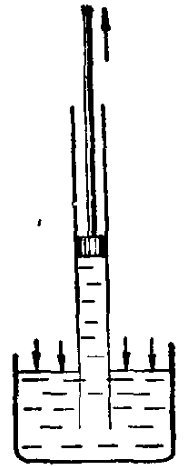
\includegraphics[width=2cm]{../pic/czwl1-ch5-46}
    \caption{大气压使水随活塞上升}\label{fig:5-46}
    \end{minipage}
    \qquad
    \begin{minipage}{7cm}
    \centering
    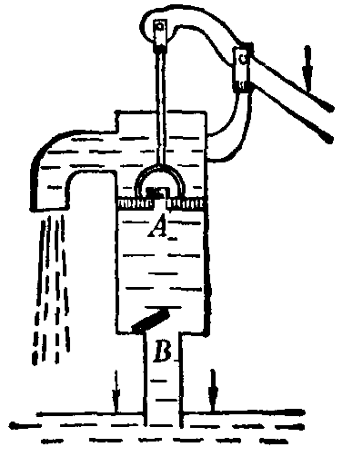
\includegraphics[width=4cm]{../pic/czwl1-ch5-47}
    \caption{吸取式抽水机}\label{fig:5-47}
    \end{minipage}
\end{figure}

图 \ref{fig:5-47} 是一种活塞式抽水机的示意图。这种抽水机叫做吸取式抽水机。
它的进水管插在水井中,上面的圆筒里装着一个跟筒壁配合得很紧密的活塞,筒底和活塞上各有一个只能向上开的阀门。
提起活塞的时候,阀门 $A$ 关闭,大气压使水推开阀门 $B$ 进入圆筒中。
压下活塞的时候,活塞下面的水压在阀门 $B$ 上,使阀门 $B$ 关闭,水不能往下跑,就推开阀门 $A$ 进到活塞上面。
再提起活塞,活塞上面的水使阀门 $A$ 关闭,水不能往下跑,就被活塞提起,从侧管中排出去。
同时井里的水又在大气压的作用下推开阀门 $B$ 进入圆筒中。
活塞这样上下往复运动,就不断把水抽上来了。

\begin{wrapfigure}[16]{r}{5.5cm}
    \centering
    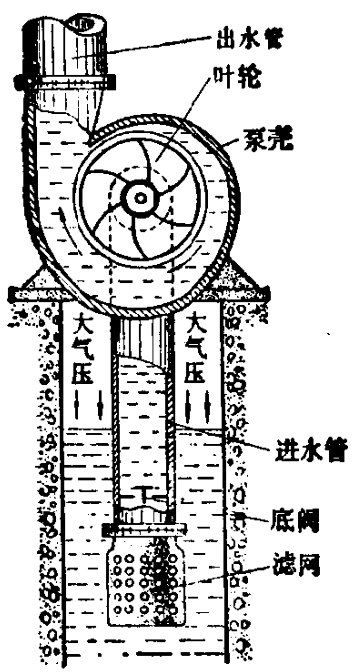
\includegraphics[width=5cm]{../pic/czwl1-ch5-48}
    \caption{离心泵示意图}\label{fig:5-48}
\end{wrapfigure}
活塞式抽水机的结构简单,操作方便,主要用在生活中。
但是,它的出水量小,提水高度小,效率也低。
在生产中需要大量提水的时候,广泛使用的是离心式水泵。

离心式水泵通常叫做离心泵,图 \ref{fig:5-48} 是它的示意图。
它的主要部分是泵壳和装在泵壳里面的叶轮。水泵起动前,先往泵壳里灌满水。
起动后,叶轮在动力机的带动下旋转。泵壳里的水也跟着旋转,同时被叶轮甩入出水管中。
水被甩出时,叶轮附近的压强减小,比大气压小得多,因此进水管外面的水就在大气压的作用下,
推开底阀通过进水管进入泵壳里,进来的水在随叶轮旋转时又被甩入出水管中。
叶轮不停地旋转,就把水不断地从低处抽到高处。


\nonumsection{阅读材料:大气压发现的历史}

大气压强的发现是与抽水机紧密相联的。

在很古的时候,人们就已经会用图 \ref{fig:5-47} 那样的抽水机抽水了,
那时人们用“自然害怕真空”来解释水在抽水机中随活塞上升的现象。
对这种现象的真正原因——大气压强是不知道的。

1640 年,随着生产的发展,在当时意大利的繁华商业城市佛罗伦萨制造了一个很高的抽水机,
想用它来抽出深矿坑中的水。但是,把抽水机安装好并用来抽水以后,却发现水只能吸到大约 10 米的高度。
技师们想了各种办法使活塞和筒壁间紧密配合,但是仍然不能使水上升得更高。

技师们去向当时的大科学家伽利略求教,伽利略已经年老多病,没有精力来仔细研究这个问题。
但是他指出,如果水在抽水机中能够升高 10 米,那么比水轻的油就应该升高得多一些,
而比水重得多的水银升高的高度则应该比 10 米少得多。

伽利略去世后,他的学生托里拆利继续研究这个问题。
他用玻璃管代替不透明的金属圆筒,用水银代替水做实验。
结果跟伽利略预料的完全相符,水银在玻璃管内上升的高度仅是水上升的高度的十四分之一左右。
在托里拆利实验中,玻璃管内水银的上方就是真空,可见在自然界中是可以产生真空的,所谓“自然害怕真空” 的说法是不科学的。
托里拆利的实验不但揭示了大气压的存在,而且测出了大气压的值。

因为大气压有一定的大小,所以水在抽水机中上升的高度有一定的限度,即 10 米左右。



\lianxi

(1) 登山运动员在上升到高山上时,常产生许多不舒服的感觉,叫做高山反应,产生这种反应的原因是什么?

(2) 1 标准大气压能支持多高的水柱?

(3) 活塞式抽水机的活塞和筒壁间如果配合不紧,就抽不上水来,这是为什么?

(4) 使用离心式水泵,起动前如果不先往泵壳里灌满水,水泵能抽上水来吗?为什么?



\nonumsection{小实验:研究大气压和天气的关系}

每天上下午各用气压计测量一次大气压,把所得数据记录下来,并在方格纸上画出气压变化的曲线,
每星期小结一次,研究大气压的值和天气晴、雨的关系。

